\documentclass[thesis.tex]{subfiles}
\chapter{Mô hình xác minh người nói tiếng Việt}
Trong chương này, tác giả trình bày mô hình học sâu cơ sở giải quyết bài toán xác minh người nói, đề xuất phương pháp để cải tiến mô hình cho tiếng Việt và trình bày các nghiên cứu liên quan.

\section{Mô hình cơ sở}\label{baseline}

\begin{figure}[h]
    \centering
    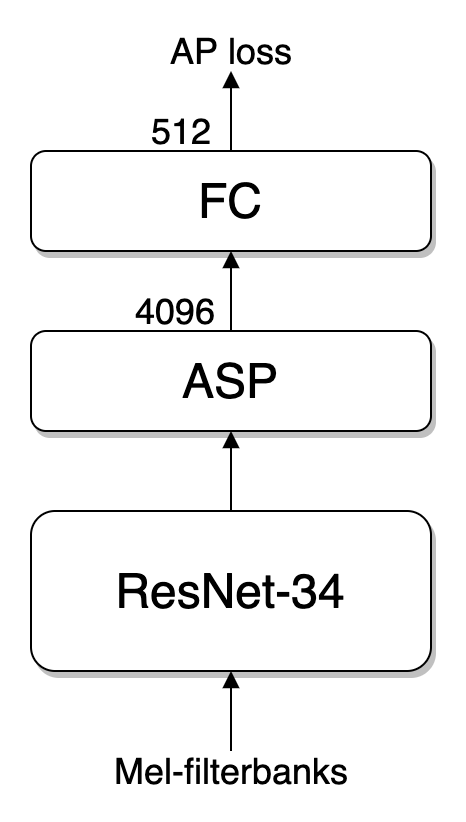
\includegraphics[width=0.3\textwidth]{images/ap-resnet.png}
    \caption{Tổng quan mô hình cơ sở sử dụng trong đồ án.}
    \label{fig:ap-resnet}
\end{figure}

Mô hình cơ sở \cite{heo2020clova} là mô hình tốt nhất cho xác minh người nói tại thời điểm hiện tại được sử dụng trong đồ án tuân theo hệ thống ba pha được mô tả như trong phần \ref{related-works} (Hình \ref{fig:ap-resnet}). Mô hình nhận đầu vào là một mini-batch các đặc trưng âm học của nhiều câu nói khác nhau. Mạng ResNet-34 trích xuất biểu diễn của các đặc trưng đầu vào; do mỗi câu nói có nhiều khung, mô hình sử dụng một lớp tổng hợp thống kê tập trung (Attentive Statistic Pooling - ASP) để giúp biểu diễn câu nói luôn có chiều cố định. Cuối cùng, giá trị mất mát của một mini-batch được tính toán bằng hàm mất mát nguyên mẫu góc (Angular Prototypical - AP). Toàn bộ mô hình được cập nhật cho mỗi mini-batch sử dụng lan truyền ngược và phương pháp tối ưu Adam.

Trong các mục tiếp theo, đồ án sẽ trình bày chi tiết các thành phần chính của mô hình.

\subsection{Biểu diễn khung giọng nói bằng mạng ResNet}
Mạng ResNet sử dụng trong đồ án là biến thể của mạng ResNet-34 như mô tả trong phần \ref{deep-learning}. Tại mỗi lớp, mạng sử dụng một nửa số bộ lọc so với mạng ResNet-34 gốc trong các khối ResNet và chứa tổng cộng 8.0 triệu trọng số. Trong lớp tích chập đầu tiên, tham số bước nhảy được chỉnh thành 1 so với 2 trong mạng ResNet-34 gốc khiến đầu vào của các lớp đằng sau lớn hơn từ đó tăng khối lượng tính toán. Chi tiết cấu trúc của mạng được mô tả trong Bảng \ref*{tab:resnet-34}.

\begin{table}[h]
    \centering
    \begin{tabular}{l c c c}
      \hline
      \textbf{Layer}& \textbf{Kernel size} & \textbf{Stride} & \textbf{Output shape} \\
      \hline
      Conv1       & $3 \times 3 \times 32$   & 1 $\times$ 1  & $L \times 64 \times 32$ \\
      \hline
      ResBlock1   & $3 \times 3 \times 32$   & 1 $\times$ 1  & $L \times 64 \times 32$ \\
      \hline
      ResBlock2   & $3 \times 3 \times 64$  & 2 $\times$ 2   & $L/2 \times 32 \times 64$ \\
      \hline
      ResBlock3   & $3 \times 3 \times 128$  & 2 $\times$ 2  & $L/4 \times 16 \times 128$ \\
      \hline
      ResBlock4   & $3 \times 3 \times 256$  & 2 $\times$ 2  & $L/8 \times 8 \times 256$ \\
      \hline
      Flatten     & -  & -  & $L/8 \times 2048$ \\
      \hline
    \end{tabular}
    \caption{Kiến trúc mạng ResNet sử dụng trong đồ án}
    \label{tab:resnet-34}
\end{table}

% \TODO{input output of network}

\subsection{Tổng hợp thống kê tập trung}
Trong thực tế, không phải khung âm thanh nào cũng chứa nhiều thông tin của người nói do độ dài một khung rất ngắn thông thường chỉ 25 mili giây. Ví dụ, một khung có thể chứa nhiều tiếng ồn, hoặc không hề chứa giọng nói. Do vậy, hệ thống sử dụng tổng hợp thống kê tập trung để đánh trọng số cho biểu diễn của các khung với mong muốn tăng thông tin của những khung nhiều ý nghĩa và giảm thông tin của những khung ít ý nghĩa. Từ đó có thể phân biệt giọng nói một cách hiệu quả hơn.

ASP \cite{okabe2018attentive} nhận đầu vào là tập các vec-tơ biểu diễn khung $\bm{h}_t\ (t=1,...,T)$. Vec-tơ biểu diễn của toàn đoạn âm thanh được tính qua 2 bước: đánh trọng số cho từng khung bằng cơ chế tập trung và tổng hợp thông tin thống kê dựa trên trọng số tính được (Hình \ref{fig:asp}).

\begin{figure}[h]
    \centering
    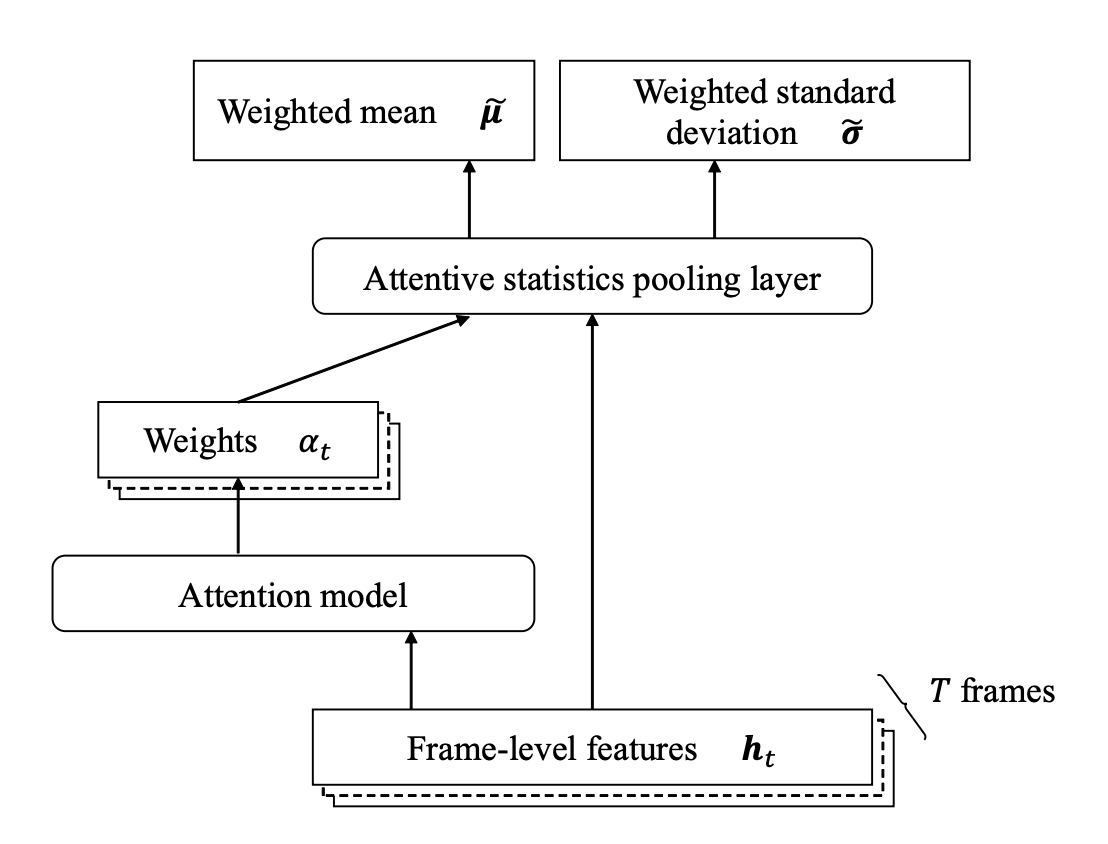
\includegraphics[width=0.7\textwidth]{images/attentive-statistic-pooling.png}
    \caption{Tổng hợp thống kê tập trung \cite{okabe2018attentive}.}
    \label{fig:asp}
\end{figure}

\subsubsection{Cơ chế tập trung}

Bằng cơ chế tập trung, trọng số của từng khung có thể được tính theo hai Công thức \ref{eq:att1} và \ref{eq:att2}.

\begin{equation} \label{eq:att1}
    e_t = \bm{v}^T f(\bm{W}\bm{h}_t + b) + k
\end{equation}

\begin{equation} \label{eq:att2}
    \alpha_t = \dfrac{\alpha_t}{\sum_\rho^T \alpha_\rho}
\end{equation}

Trong Công thức \ref{eq:att1}, với $\bm{v}, \bm{W}$ là các ma trận trọng số có thể học được, $f$ là hàm kích hoạt phi tuyến như tanh hoặc ReLu, ta tính được điểm cho mỗi khung $e_t$. Sau đó, điểm của mỗi khung được chuẩn hoá trên tất cả các khung để thu được trọng số tập trung bằng hàm softmax như trong Công thức \ref{eq:att2}.

\subsubsection{Tổng hợp thống kê}
Sau khi có được trọng số của các khung, ta tính vec-tơ trung bình có trọng số với Công thức \ref{eq:asp1}.

\begin{equation} \label{eq:asp1}
    \bm{\mu} = \sum_t^T \alpha_t\ \bm{h}_t
\end{equation}

Bằng cách tính này, vec-tơ biểu diễn của đoạn âm thanh tập trung hơn vào những khung tiếng nói có ý nghĩa cao. Ngoài ra, các trọng số tập trung còn được sử dụng để tính độ lệch chuẩn có trọng số theo Công thức \ref{eq:asp2}. 

\begin{equation} \label{eq:asp2}
    \bm{\sigma} = \sqrt{\sum_t^T \alpha_t \bm{h}_t \odot \bm{h}_t - \bm{\mu} \odot \bm{\mu}}
\end{equation}

Với $\odot$ là phép nhân Hadamard, $\bm{\mu}$ là vec-tơ trung bình có trọng số tính trong Công thức \ref{eq:asp1}. Sau khi hoàn tất quá trình tính toán vec-tơ trung bình và độ lệch chuẩn có trọng số, $\bm{\mu}$ và $\bm{\sigma}$ được ghép lại để biểu diễn cho một đoạn tiếng nói. Bằng cách này, mọi đoạn âm thanh dài ngắn đều có vec-tơ biểu diễn với số chiều như nhau, được tổng hợp từ những khung âm thanh có ý nghĩa nhất trong câu.

\subsection{Hàm mất mát nguyên mẫu góc AP} \label{ap-loss}
Trong thực tế, ta cần tổng hợp từ một số câu nói nhất định để tạo vec-tơ biểu diễn người nói. Do vậy, Chung và cộng sự \cite{chung2020defence} đề xuất hàm mất mát AP tối ưu không gian biểu diễn dựa trên nguyên mẫu (prototype) của người nói. Mỗi người nói có một nguyên mẫu và một câu truy vấn, mục tiêu của AP là đẩy xa truy vấn của một người ra xa nguyên mẫu của những người khác và kéo nó lại gần nguyên mẫu của người đó (Hình \ref{fig:ap-loss}).

\begin{figure}[h]
    \centering
    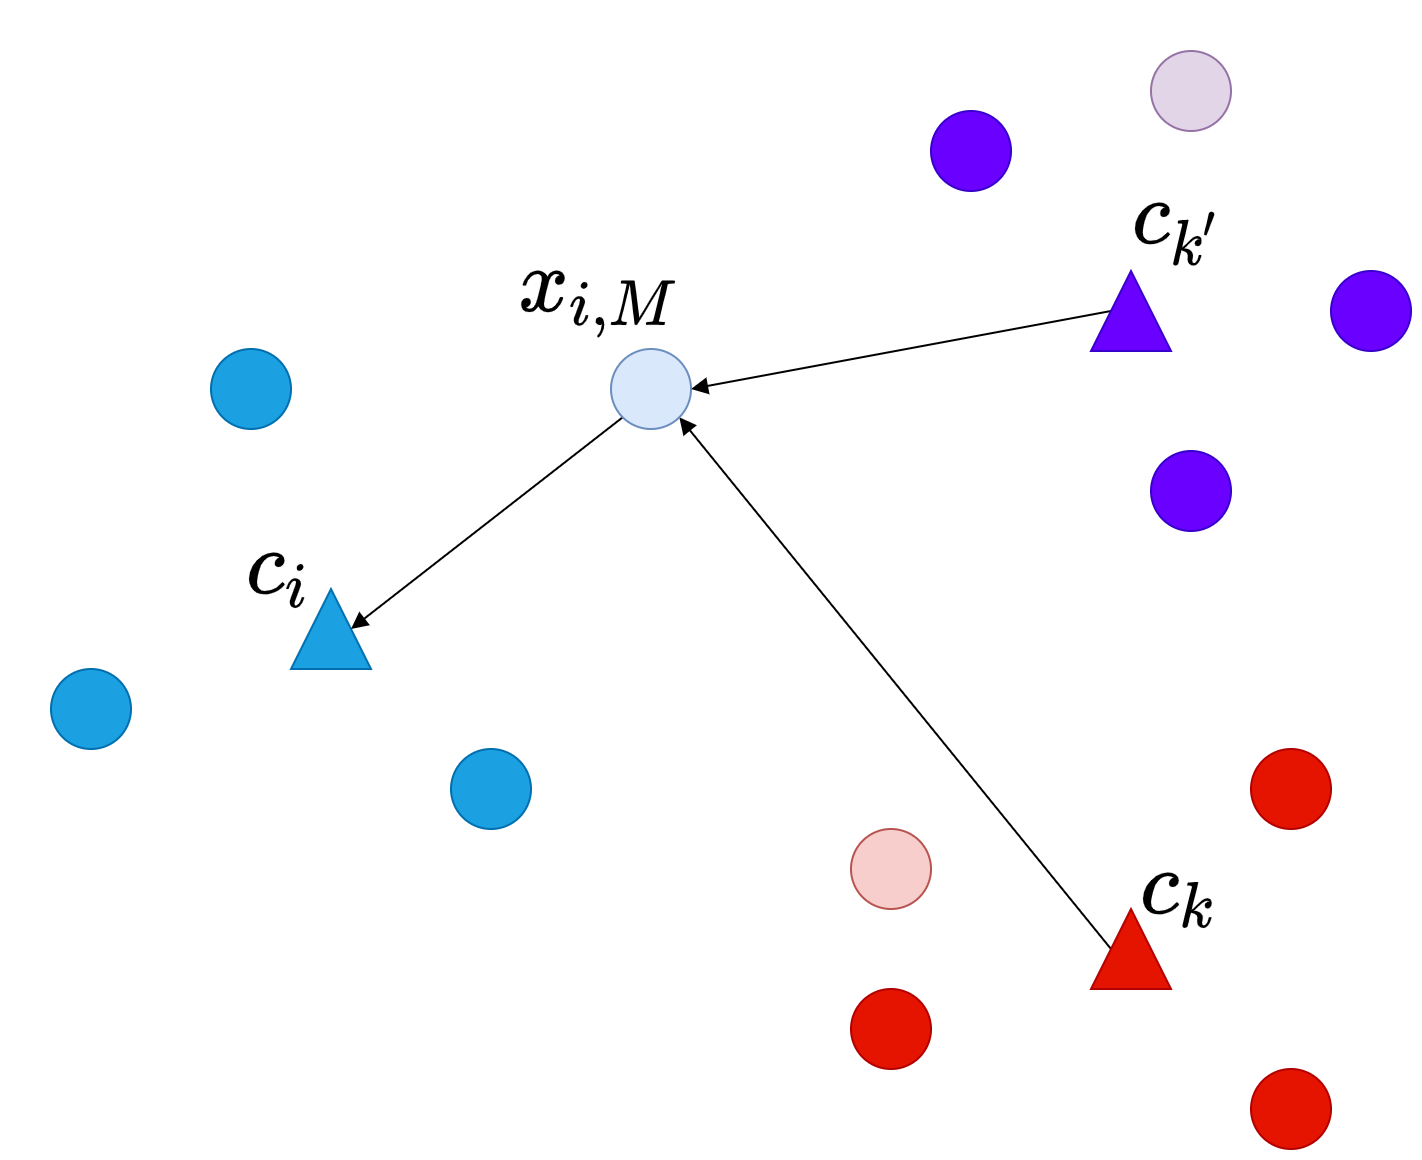
\includegraphics[width=0.6\textwidth]{images/ap-loss.png}
    \caption{Hàm mất mát Angular Prototypical.}
    \label{fig:ap-loss}
\end{figure}

Xét một mini-batch gồm $M$ đoạn tiếng nói từ mỗi $N$ người nói, gọi $\bm{x}_{i,j}$ là vec-tơ biểu diễn của đoạn tiếng nói thứ $j$ của người thứ $i$, $1 \leq i \leq N, 1 \leq j \leq M$. Giả sử truy vấn của một người là câu cuối cùng của người đó $\bm{x}_{i,M}$, nguyên mẫu của một người nói được tính toán như Công thức \ref{eq:ap1}.

\begin{equation}\label{eq:ap1}
    \bm{c}_i = \dfrac{1}{M-1}\sum_{m=1}^{M-1}\ \bm{x}_{i,m}
\end{equation}

Trong AP, độ tương đồng cô-sin được sử dụng để làm độ đo. Độ tương đồng được tính theo Công thức \ref{eq:cosine} với hệ số scale $w$ và bias $b$. Hai hệ số này giúp mô hình hội tụ ổn định hơn và khái quát hoá tốt hơn với thay đổi trong đặc trưng đầu vào \cite{wang2017deep}.

\begin{equation}\label{eq:cosine}
    \bm{S}_{i,k} = w \cdot cos(\bm{x}_{i,M}, \bm{c}_k) + b
\end{equation}

Trong quá trình huấn luyện, câu truy vấn của mỗi người được phân loại dựa trên độ tương đồng đối với $N$ nguyên mẫu trong mini-batch:

\begin{equation}\label{eq:nll-softmax}
    L_{AP} = - \dfrac{1}{N} \sum_{i=1}^N log \dfrac{e^{\bm{S}_{i,i}}}{\sum_{k=1}^N e^{\bm{S}_{i,k}}}
\end{equation}

Trong Công thức \ref*{eq:nll-softmax}, $\bm{S}_{i, i}$ là độ tương đồng của truy vấn người $i$ và nguyên mẫu của chính người đó. Bằng việc sử dụng hàm softmax, $\bm{S}_{i,i}$ được đẩy gần hơn tới 1 và mô hình bị "phạt" nặng hơn nếu độ tương đồng của truy vấn người $i$ tới nguyên mẫu của người khác lớn.

\section{Đề xuất mô hình cho tiếng Việt}\label{propose}
\subsection{Mô hình tổng quan}
Như đã trình bày trong phần \ref{vietnamese-speaker-recognition}, dữ liệu tiếng Việt còn rất hạn chế, vì vậy đồ án đề xuất mô hình dựa trên học chuyển tiếp nhằm tận dụng kiến thức từ lượng dữ liệu khổng lồ có trong tiếng Anh. Hình \ref{fig:overall-propose} mô tả tổng quan mô hình đề xuất. Tương tự mô hình cơ sở, mô hình nhận đầu vào là một mini-batch đặc trưng âm học của các câu nói từ nhiều người khác nhau. Mạng ResNet-34 được khởi tạo với trọng số từ mô hình tiếng Anh huấn luyện trên VoxCeleb để học chuyển tiếp. ASP cũng được sử dụng bởi mô hình nhằm tổng hợp biểu diễn khung. Tiếp theo, giá trị mất mát được tính toán với hàm mất mát nguyên mẫu góc với hệ số phạt biên (Angular Margin Prototypical - AMP). Bộ trọng số của mô hình được cập nhật với hàm tối ưu SGD thay cho Adam. Trong các mục tiếp theo trong chương này, đồ án trình bày chi tiết về các thay đổi của mô hình đề xuất so với mô hình đề xuất: học chuyển tiếp, hàm mất mát và phương pháp tối ưu.

\begin{figure}[h]
    \centering
    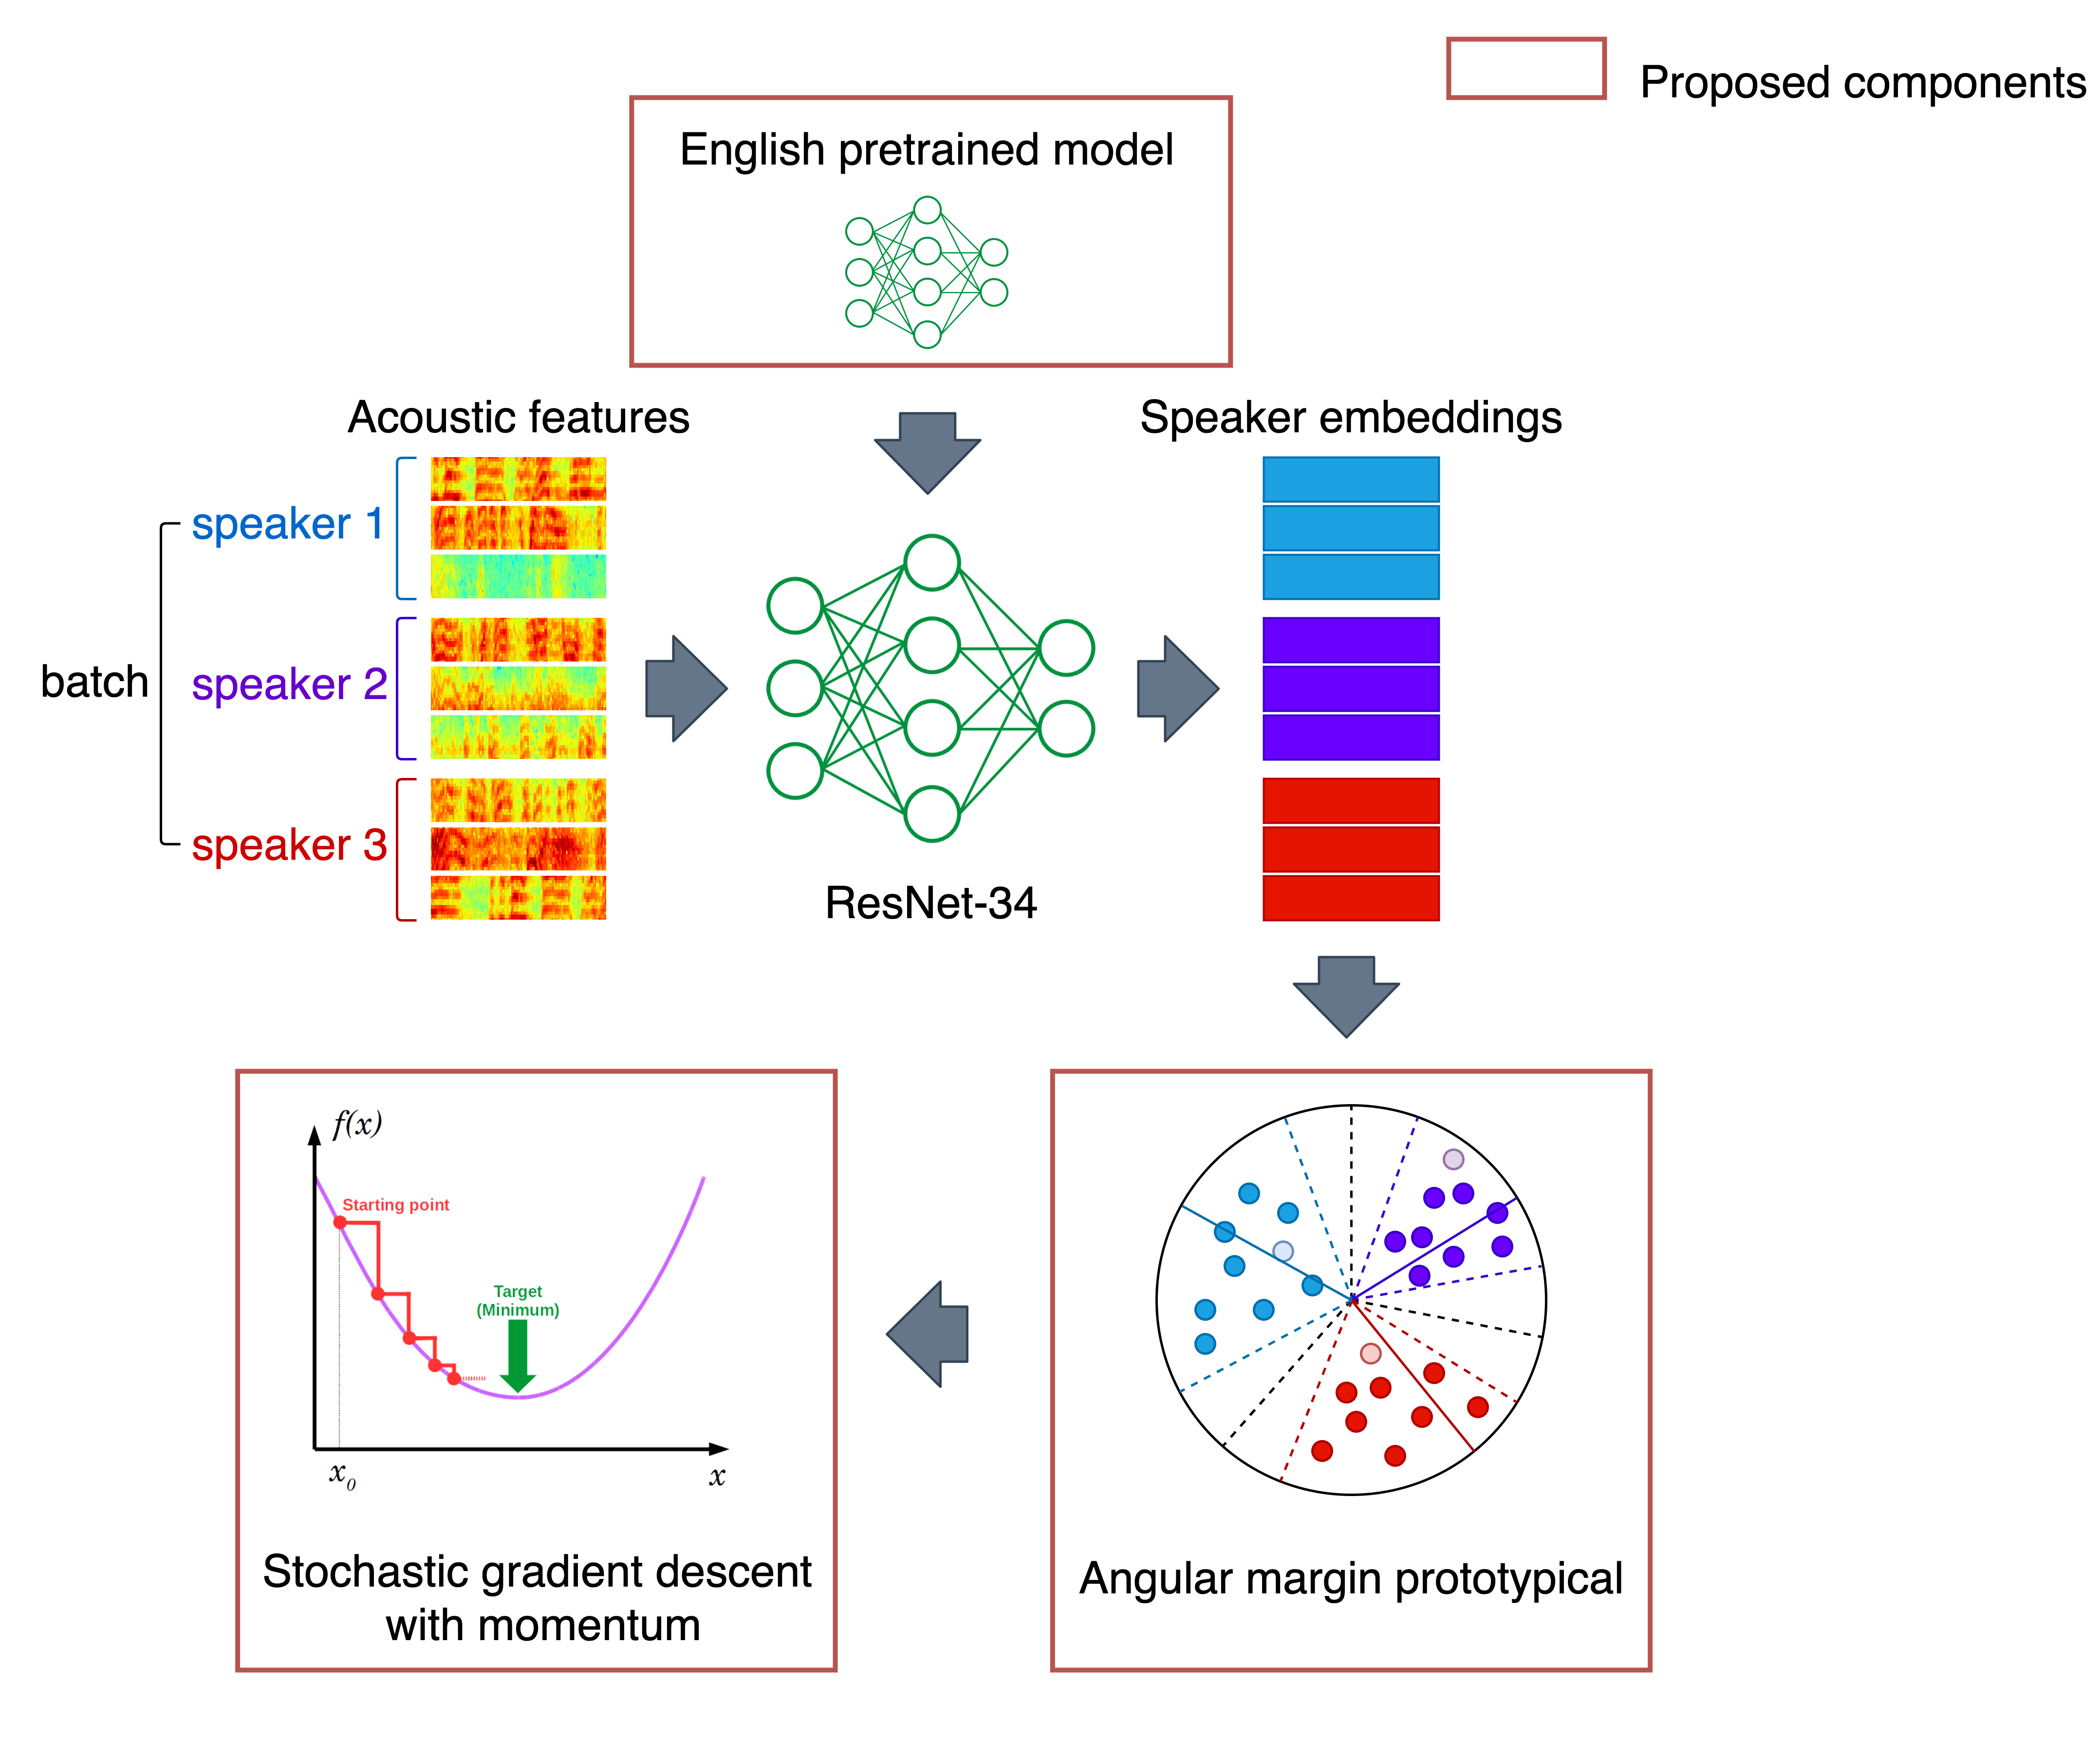
\includegraphics[width=0.9\textwidth]{images/overall-propose.png}
    \caption{Tổng quan phương pháp đề xuất cho xác minh người nói tiếng Việt.}
    \label{fig:overall-propose}
\end{figure}

\subsection{Học chuyển tiếp sử dụng kiến thức trên tiếng Anh}
Học chuyển tiếp là một kỹ thuật trong học máy khi mà một mô hình được huấn luyện cho một tác vụ nhất định được sử dụng làm điểm bắt đầu cho một tác vụ khác. Học chuyển tiếp cho phép rút ngắn quá trình huấn luyện và gia tăng hiệu năng cho quá trình huấn luyện mô hình trên tác vụ mới với ít dữ liệu hơn đáng kể. 

\begin{figure}[h]
    \centering
    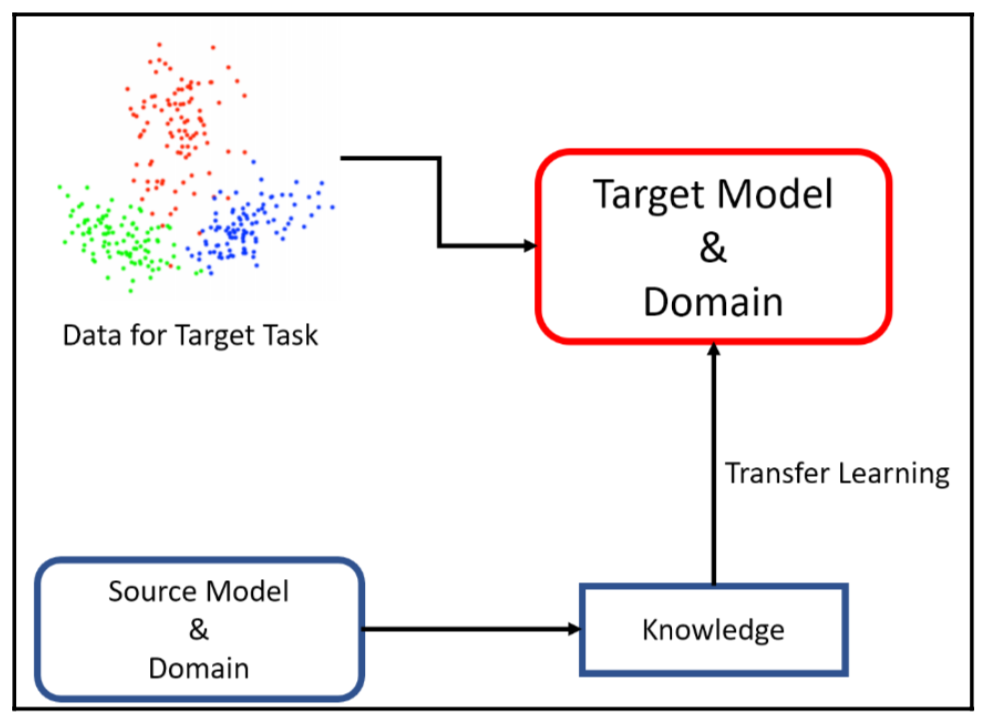
\includegraphics[width=0.65\textwidth]{images/transfer-learning.png}
    \caption{Sơ đồ mô tả học chuyển tiếp sử dụng kiến thức hiện có cho các tác vụ mới \cite{sarkar2018hands}.}
    \label{fig:transfer-learning}
\end{figure}

Cụ thể hơn, học chuyển tiếp hỗ trợ việc huấn luyện tác vụ mục tiêu theo những cách sau: 

\begin{itemize}
    \item Hiệu suất cơ sở tốt hơn (higher start): khi ta tăng cường kiến thức của mô hình mới với kiến thức từ mô hình gốc, hiệu suất cơ sở có thể cải thiện nhờ việc chuyển giao kiến thức.
    \item Thời gian huấn luyện ngắn hơn (higher slope): tốc độ hội tụ của mô hình mới có thể nhanh hơn dẫn tới thời gian huấn luyện ngắn hơn.
    \item Kết quả cuối cùng tốt hơn (higher asymptote): hiệu suất cuối cùng cao hơn có thể đạt được bằng việc sử dụng học chuyển tiếp.
\end{itemize}

\begin{figure}[h]
    \centering
    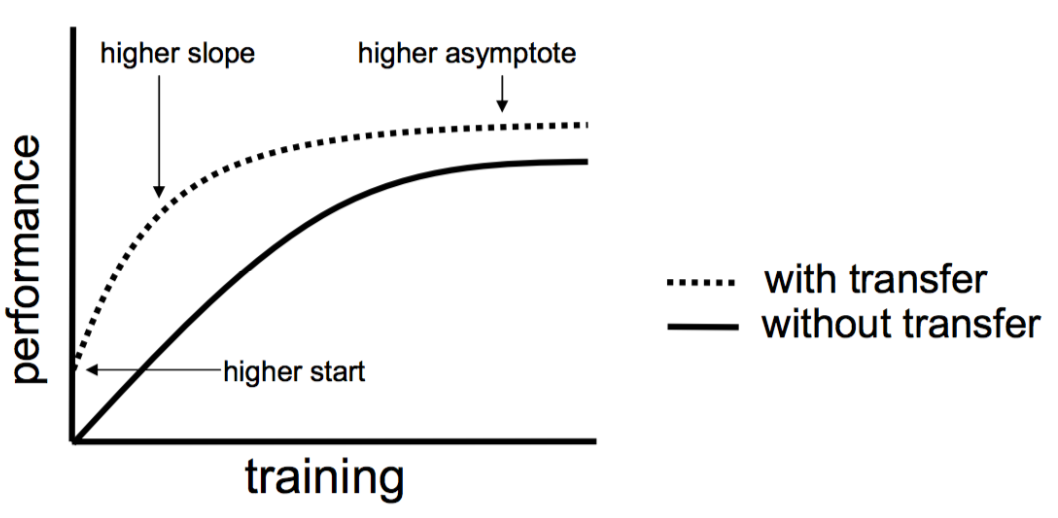
\includegraphics[width=0.7\textwidth]{images/transfer-learning-benefits.png}
    \caption{Lợi ích của học chuyển tiếp đối với việc huấn luyện mô hình \cite{aytar2011tabula}.}
    \label{fig:transfer-learning-benefits}
\end{figure}

Huấn luyện mô hình học sâu cần một lượng lớn tài nguyên tính toán và dữ liệu, do đó học chuyển tiếp được sử dụng rộng rãi trong cộng đồng nghiên cứu học sâu cho bài toán thị giác máy tính hay xử lý ngôn ngữ tự nhiên. Các thư viện học sâu nổi tiếng như Pytorch hay Tensorflow đều công bố các mô hình huấn luyện sẵn trên hàng triệu hay chục triệu ảnh giúp cộng đồng phát triển các mô hình học sâu dễ dàng và hiệu quả hơn với ít dữ liệu. Gần đây, cộng đồng nghiên cứu xử lý ngôn ngữ tự nhiên cũng có thể lợi dụng các mô hình huấn luyện sẵn cực lớn với hàng trăm tỉ trọng số như BERT \cite{devlin2018bert}, GPT-2 \cite{radford2019language} hay GPT-3 \cite{brown2020language} để cải tiến các tác vụ hạ lưu như phân loại nhận dạng thực thể, phân tích cú pháp phụ thuộc, tóm tắt văn bản, ...

Trong đồ án, phương pháp học chuyển tiếp từ mô hình huấn luyện trên người nói tiếng Anh được áp dụng để cải thiện mô hình giọng nói tiếng Việt. Mặc dù âm điệu hay đặc điểm của người nói tiếng Anh khác nhiều so với tiếng Việt, kiến thức về âm thanh huấn luyện trên hàng nghìn giờ dữ liệu tiếng Anh khả năng cao sẽ làm tăng cường kết quả trong tiếng Việt.

\subsection{Hàm mất mát AMP tăng tính phân tách biểu diễn người nói}
Như đã mô tả trong phần \ref{ap-loss}, hàm mất mát AP khuyến khích biểu diễn câu nói của một người gần hơn tới nguyên mẫu $\bm{c}_i$ của người đó hơn là các nguyên mẫu khác. Tuy vậy, khoảng cách giữa các câu nói của một người còn khá lớn và các câu khác người nói ở gần biên quyết định hàm softmax có khoảng cách nhỏ. Đây cũng là điểm yếu của hàm softmax mà nhiều nghiên cứu trước đây cũng đã chỉ ra. Biên quyết định yếu có thể gây ra tỉ lệ nhầm lẫn cao khi triển khai mô hình trong thực tế.

\begin{figure}[h]
    \centering
    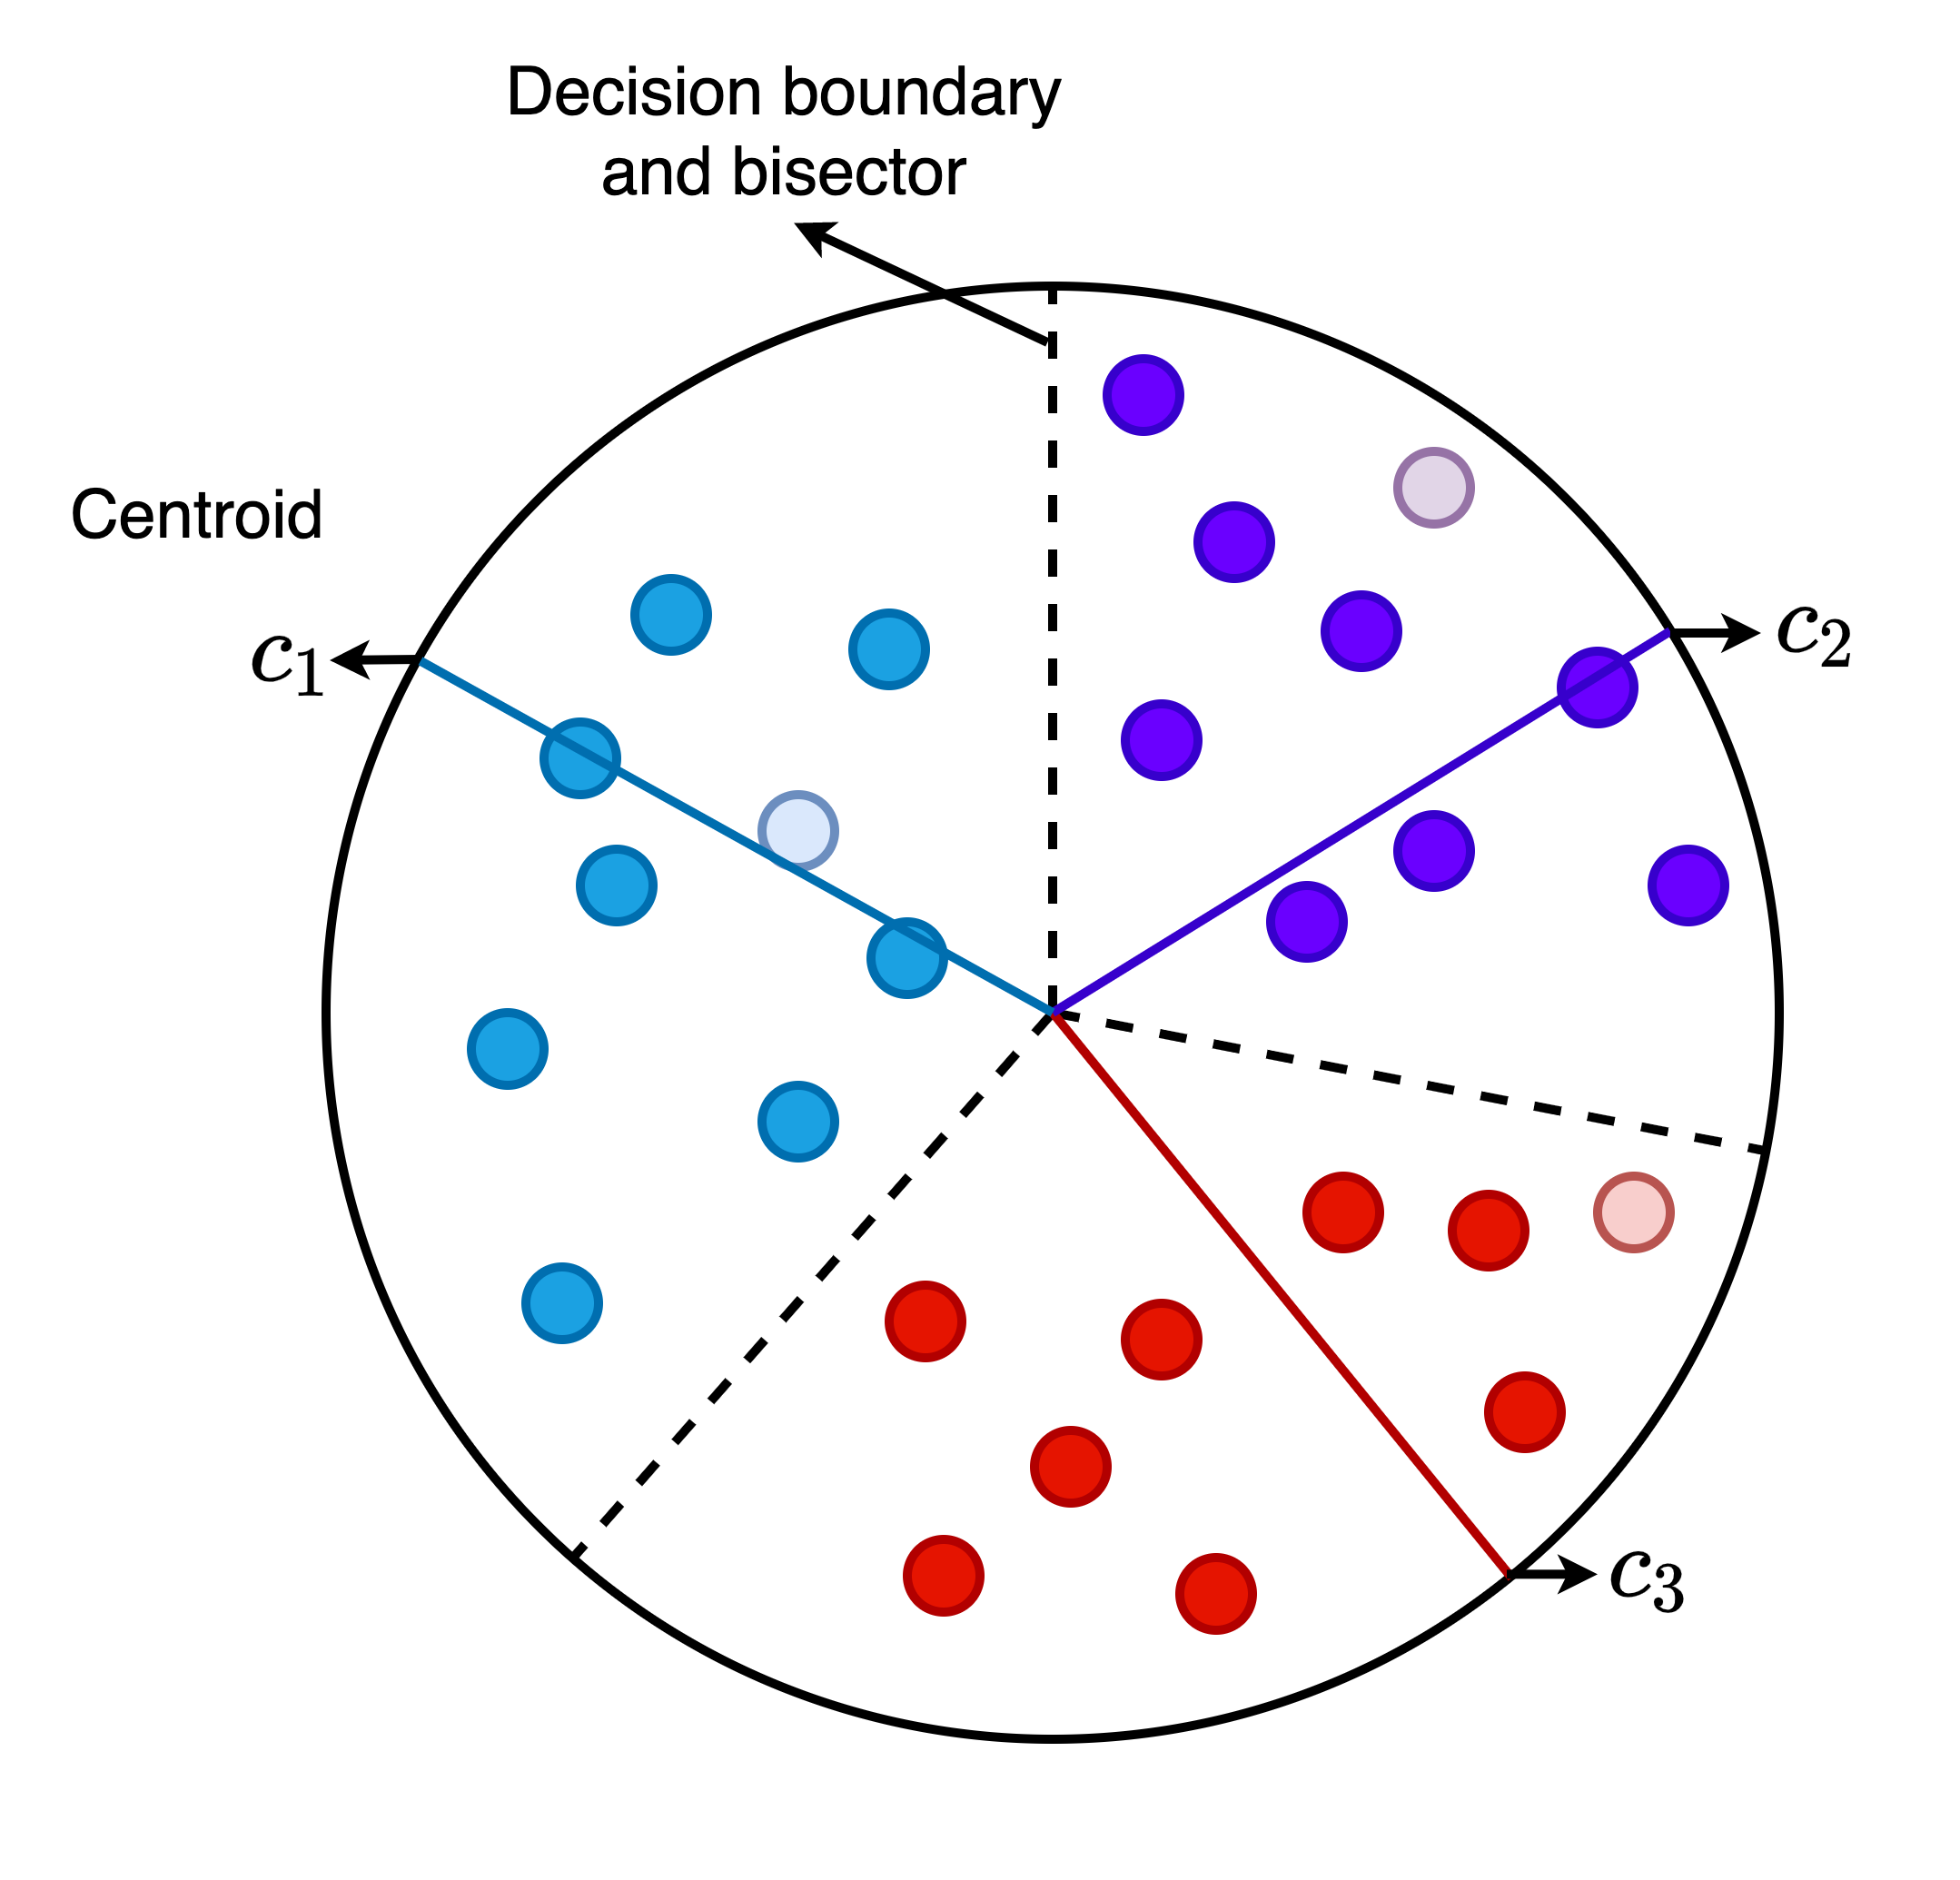
\includegraphics[width=0.54\textwidth]{images/softmax-angular-space.png}
    \caption{Mô tả biểu diễn người nói học bởi hàm softmax trong không gian góc. Đường kẻ chấm đen là đường phân giác giữa 2 tâm.}
    \label{fig:softmax-angular-space}
\end{figure}

Nhận thấy sự hiệu quả của việc dùng hệ số phạt biên trong các hàm mất mát phân loại như AM-Softmax \cite{wang2018additive} hay \cite{deng2019arcface}, tác giả đề xuất hàm mất mát Angular Margin Prototypical (AMP) thêm hệ số phạt biên vào hàm AP. Hàm AMP có thể được chia thành 2 loại AMP-cos hoặc AMP-arc phụ thuộc vào cách thêm hệ số phạt vào điểm tương đồng cô-sin hoặc góc giữa điểm biểu diễn và nguyên mẫu.

\subsubsection{AMP-cos}
Trong hàm AMP-cos, hệ số phạt biên được thêm trực tiếp vào điểm tương đồng của 2 câu. Công thức tính điểm tương đồng \ref{eq:cosine} được viết trong Công thức \ref{eq:cosine-cos}.

\begin{equation} \label{eq:cosine-cos}
    \bm{S}_{i, k} = 
\begin{cases}
    w \cdot (\cos \left(\theta_{\bm{x}_{i, M}, \bm{c}_{k}}\right) - m)+b, & \text{nếu } i = k\\
    w \cdot \cos \left(\theta_{\bm{x}_{i, M}, \bm{c}_{k}}\right)+b,              & \text{ngược lại}
\end{cases}
\end{equation}

trong đó $\theta_{\bm{x}_{i, M}, \bm{c}_{k}}$ là góc giữa truy vấn $\bm{x}_{i, M}$ của người $i$ và nguyên mẫu $\bm{c}_{k}$ của người $k$, $w$ và $b$ là các trọng số học được, và $m$ là hệ số phạt biên. Thay vào Công thức \ref{eq:nll-softmax}, ta được hàm mất mát AMP-cos như trong \ref{eq:amp-cos}.

\begin{equation} \label{eq:amp-cos}
    L_{AMP-cos} = - \dfrac{1}{N} \sum_{i=1}^N log \dfrac{e^{w \cdot (\cos \left(\theta_{\bm{x}_{i, M}, \bm{c}_{i}}\right) - m)+b}}{e^{w \cdot (\cos \left(\theta_{\bm{x}_{i, M}, \bm{c}_{i}}\right) - m)+b} + \sum_{k=1, k \neq i}^N e^{w \cdot \cos \left(\theta_{\bm{x}_{i, M}, \bm{c}_{k}}\right)+b}}
\end{equation}

\subsubsection{AMP-arc}
Hệ số phạt biên được thêm vào góc giữa 2 câu trong hàm AMP-arc. Công thức tính điểm tương đồng \ref{eq:cosine} được thay đổi như trong Công thức \ref{eq:cosine-arc}.

\begin{equation} \label{eq:cosine-arc}
    \bm{S}_{i, k} = 
\begin{cases}
    w \cdot \cos \left(\theta_{\bm{x}_{i, M}, \bm{c}_{k}} + m\right)+b, & \text{nếu } i = k\\
    w \cdot \cos \left(\theta_{\bm{x}_{i, M}, \bm{c}_{k}}\right)+b,              & \text{ngược lại}
\end{cases}
\end{equation}

Thay công thức trên vào \ref{eq:nll-softmax}, ta được hàm mất mát AMP-arc như Công thức \ref{eq:amp-arc}.

\begin{equation} \label{eq:amp-arc}
    L_{AMP-arc} = - \dfrac{1}{N} \sum_{i=1}^N log \dfrac{e^{w \cdot \cos \left(\theta_{\bm{x}_{i, M}, \bm{c}_{i}} + m\right)+b}}{e^{w \cdot \cos \left(\theta_{\bm{x}_{i, M}, \bm{c}_{i}} + m\right)+b} + \sum_{k=1, k \neq i}^N e^{w \cdot \cos \left(\theta_{\bm{x}_{i, M}, \bm{c}_{k}}\right)+b}}
\end{equation}

\begin{figure}[h]
    \centering
    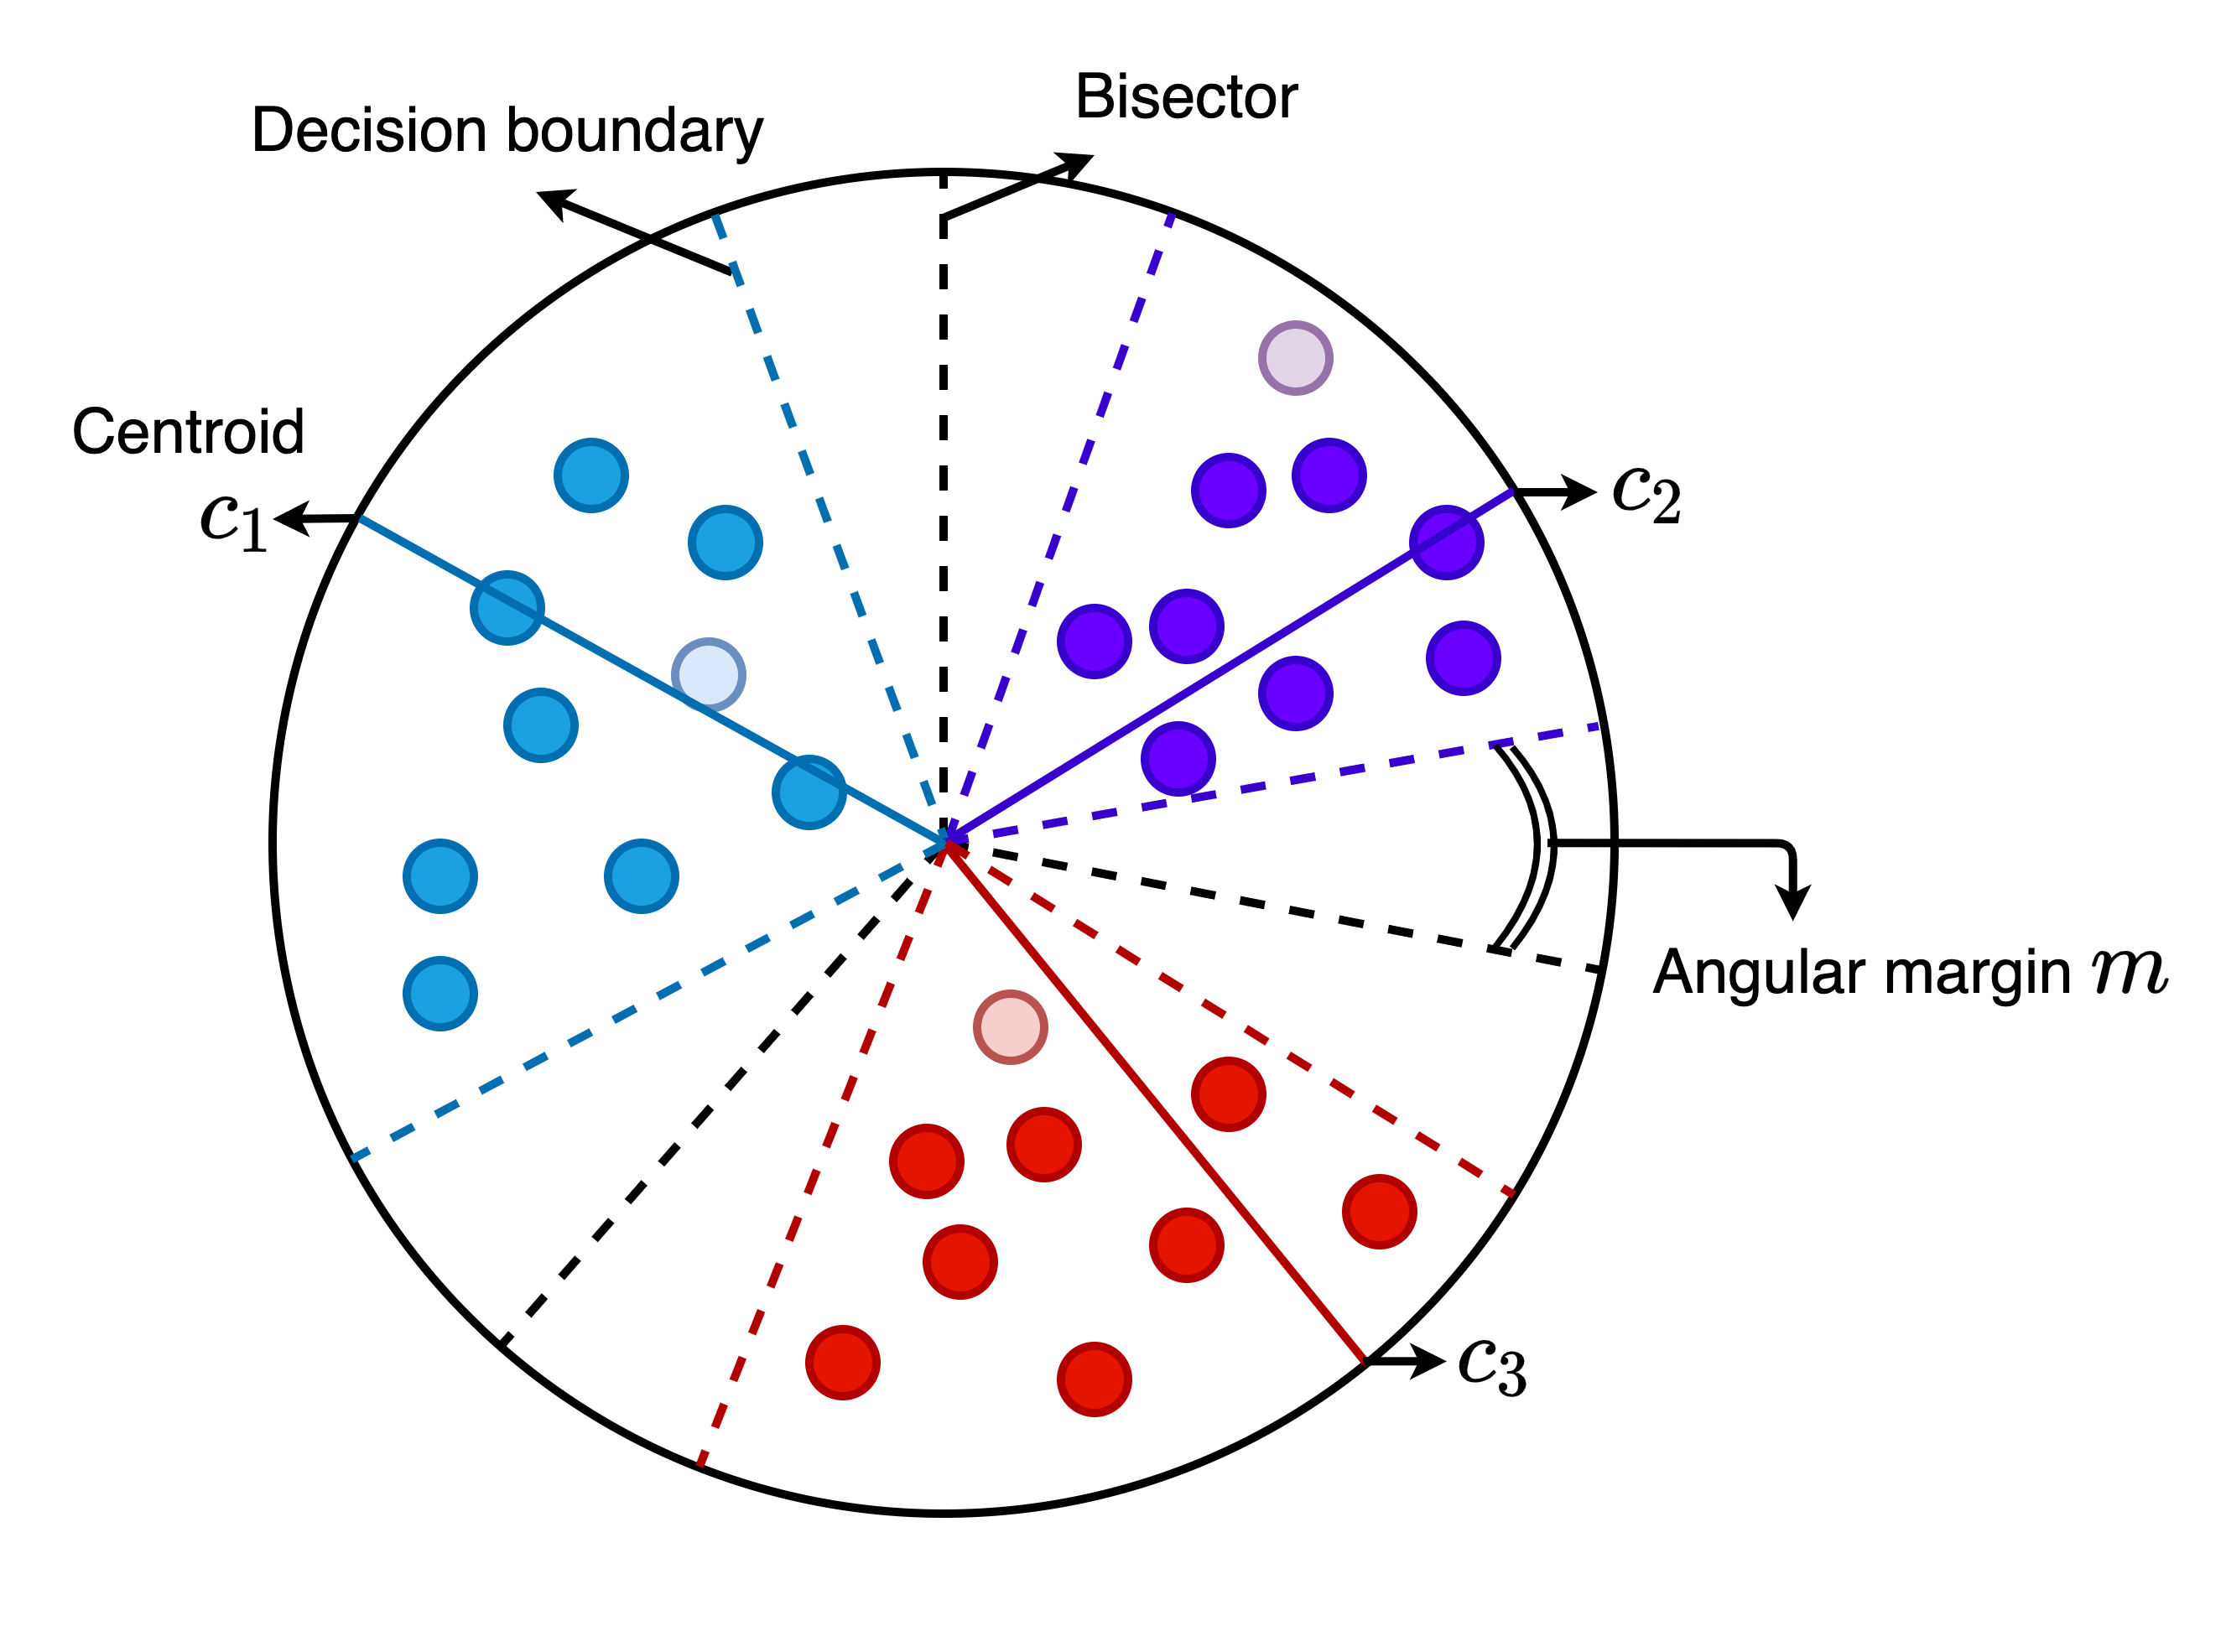
\includegraphics[width=0.65\textwidth]{images/margin-angular-space.png}
    \caption{Mô tả biểu diễn người nói học bởi hàm AMP-arc trong không gian góc.}
    \label{fig:margin-angular-space}
\end{figure}

Sự co cụm của các câu người nói (intra-class compactness) và khoảng cách với các người nói khác (inter-class separability) là 2 yếu tố chính đóng góp cho khả năng phân biệt biểu diễn người nói trong không gian vec-tơ. Việc thêm hệ số phạt biên trực tiếp làm tăng khoảng cách giữa các người nói và gián tiếp làm co cụm vùng biểu diễn của một người (Hình \ref{fig:margin-angular-space}). 

\begin{figure}[h]
    \centering
    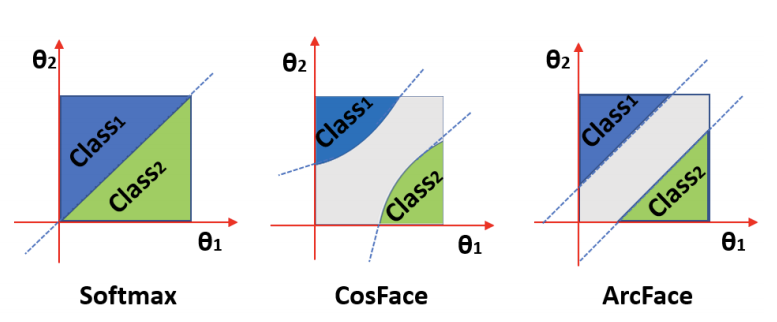
\includegraphics[width=0.65\textwidth]{images/arcface.png}
    \caption{Biên quyết định của các hàm khác nhau trong phân loại nhị phân \cite{schroff2015facenet}.}
    \label{fig:arcface}
\end{figure}

Theo các tác giả của hàm ArcFace \cite{deng2019arcface}, thiết kế hệ số phạt theo các cách khác nhau có ảnh hưởng rất lớn trong quá trình huấn luyện mô hình. Hàm AMP-arc lấy cảm hứng từ hàm ArcFace có thuộc tính hình học tốt hơn hàm AMP-cos do nó có sự tương ứng chính xác với khoảng cách trong không gian góc. Hình \ref{fig:arcface} cho thấy trong trường hợp phân loại nhị phân, hàm arc biên quyết định tuyến tính trong toàn không gian trong khi hàm cos có biên quyết định phi tuyến tính.

\subsection{SGD khái quát hoá tốt hơn Adam}
Adam \cite{kingma2014adam} là một thuật toán tối ưu thích nghi hệ số học. Được công bố vào năm 2014, Adam được trình bày tại một hội nghị rất uy tín cho cộng đồng học sâu - ICLR 2015. Bài báo phát triển một thuật toán rất hứa hẹn, cho thấy sự hội tụ vượt trội so với các thuật toán hiện hành, dẫn đến tăng tốc trong quá trình huấn luyện. 
 
Adam thích nghi hệ số học cho một trọng số của mạng sử dụng giá trị trung bình trượt của gradient và gradient bình phương của trọng số đó qua các mini-batch. Cho các trọng số $w^{(t)}$ và hàm mất mát $L^{(t)}$, trong đó $t$ là chỉ số vòng lặp trong quá trình huấn luyện, việc cập nhật trọng số trong Adam như Công thức \ref{eq:adam}.

\begin{equation} \label{eq:adam}
    \begin{split}
    m_{w}^{(t+1)} \leftarrow \beta_{1} m_{w}^{(t)}+\left(1-\beta_{1}\right) \nabla_{w} L^{(t)} \\
    v_{w}^{(t+1)} \leftarrow \beta_{2} v_{w}^{(t)}+\left(1-\beta_{2}\right)\left(\nabla_{w} L^{(t)}\right)^{2} \\ 
    \hat{m}_{w}=\frac{m_{w}^{(t+1)}}{1-\beta_{1}^{t+1}} \\ 
    \hat{v}_{w}=\frac{v_{w}^{(t+1)}}{1-\beta_{2}^{t+1}} \\
    w^{(t+1)} \leftarrow w^{(t)}-\eta \frac{\hat{m}_{w}}{\sqrt{\hat{v}_{w}}+\epsilon}
    \end{split}
\end{equation}

trong đó $\epsilon$ là một hệ số cực bé (ví dụ $10^{-6}$) để tránh phép chia cho 0, $\beta_1$ và $\beta_2$ là hệ số quên cho giá trị trung bình trượt bậc 1 và bậc 2 tương ứng. Phương pháp tối ưu đã được sử dụng trong nhiều ứng dụng do hiệu suất cạnh tranh và khả năng hoạt động tốt mà không cần điều chỉnh các hệ số. Công thức \ref*{eq:adam} cho thấy kích thước bước nhảy của quy tắc cập nhật trong Adam bất biến với độ lớn của gradient.

Tuy nhiên sau một thời gian, cộng đồng bắt đầu nhận thấy trong một số trường hợp, Adam huấn luyện mô hình tệ hơn so với phương pháp tối ưu truyền thống SGD. Bằng thực nghiệm, nghiên cứu \cite{keskar2017improving} cho thấy Adam dù trong những vòng lặp đầu vượt trội so với SGD nhưng nhanh chóng trì trệ trong những vòng lặp sau. Wilson cùng cộng sự trong \cite{wilson2017marginal} chỉ ra rằng các phương pháp thích ứng như Adam hay Adadelta không khái quát hoá SGD sau khi thử nghiệm trên một loạt các tác vụ, không khuyến khích cộng đồng sử dụng các thuật toán thích ứng. Nhìn chung, các nghiên cứu cho thấy rằng tính khái quát hoá của Adam tệ hơn SGD.

Trong bài toán xác minh người nói, người nói trong pha kiểm tra thường không có trong tập huấn luyện, tính khái quát hoá của mô hình là đặc biệt quan trọng. Lý do chính là bởi vì môi trường trong pha kiểm thử khác nhau rất nhiều so với môi trường trong dữ liệu huấn luyện và đăng ký. Do vậy mô hình có tính khái quát hoá cao, nghĩa là ít nhạy cảm với điều kiện của môi trường cho kết quả tốt hơn.

Vì các lý do kể trên, đồ án đề xuất thay thế sử dụng SGD thay cho Adam trong mô hình cơ sở.

\section{Nghiên cứu liên quan}
Như đã trình bày trong phần \ref{propose}, mô hình đề xuất sử dụng học chuyển tiếp, hàm tối ưu SGD và thêm hệ số phạt góc cho hàm mất mát AP. Sau đây, đồ án trình bày một số nghiên cứu liên quan về các phần trong mô hình đề xuất.

% Transfer learning in speaker recognition
\textbf{Học chuyển tiếp}. Phương pháp học chuyển tiếp được ứng dụng tương đối rộng rãi cho bài toán xác minh người nói dưới nhiều dạng khác nhau, chủ yếu để giải quyết vấn đề giữ liệu trong tác vụ mới. Trong các nghiên cứu \cite{nidadavolu2019low, xia2019cross}, các tác giả sử dụng phương pháp học đối kháng với mục đích thích ứng mô hình xác minh người nói trên dữ liệu thu bằng micrô sang dữ liệu điện thoại di động, mô hình huấn luyện trên dữ liệu chứa tiếng vang sang dữ liệu sạch và mô hình trên tiếng Anh sang tiếng Trung Quốc. Điểm chung của các tập dữ liệu mục tiêu là thời lượng ít hơn rất nhiều so với tập dữ liệu gốc và không có nhãn người nói. Trong lời giải đứng nhất \cite{thienpondt2020cross} trong cuộc thi VOXSRC-20, tác giả Thienpondt sử dụng hàm mất mát HPM để thích ứng mô hình xác minh người nói tiếng Anh sang tiếng Ba Tư với bộ dữ liệu mục tiêu gồm 588 người nói cho kết quả 1.83\% EER rất tốt đối với ngôn ngữ nghèo dữ liệu.

\textbf{Hàm mất mát với hệ số phạt biên}. Việc nghiên cứu cách thêm hệ số phạt biên vào hàm mất mát phân loại nhằm tăng tính phân biệt tương đối phổ biến trong bài toán nhận dạng - xác minh mặt người. Để giải quyết điểm yếu biên quyết định yếu của softmax, các công trình \cite{liu2017sphereface, wang2018additive, deng2019arcface} đề xuất các hàm A-softmax, CosFace và ArcFace bằng cách thêm hệ số phạt biên theo các cách khác nhau. Hai hàm CosFace và ArcFace trở nên phổ biến cho bài toán xác minh người nói do cài đặt dễ dàng và hiệu năng cao \cite{chung2020defence, xiang2019margin}. 

Các hàm mất mát phân biệt dựa trên cặp hay bộ ba như RLL \cite{wang2019ranked}, LS \cite{oh2016deep} hay hàm triplet đều được thiết kế với hệ số phạt biên. Ngược lại, các hàm mất mát phân biệt vận hành trên một mini-batch nhiều câu nói như GE2E \cite{wan2018generalized}, prototypical \cite{snell2017prototypical} hay AP \cite{chung2020defence} đều không được thiết kế với hệ số phạt biên. Gần đây, tác giả Wei cùng cộng sự nghiên cứu đưa hệ số phạt biên vào hàm GE2E cho kết quả đáng mong đợi \cite{wei2020angular}.

\textbf{Phương thức tối ưu SGD}. Hiện nay, theo hiểu biết của tác giả thì chưa có nghiên cứu nào so sánh sự hiệu quả của việc sử dụng SGD thay cho Adam trong xác minh người nói. Hơn nữa các nghiên cứu thường ít bàn luận lý do tại sao lại chọn SGD hay Adam thay vì phương thước tối ưu còn lại. Tuy nhiên, một điểm chung có thể thấy là SGD thường được sử dụng để đạt kết quả hiện đại nhất (state of the art) cho các mạng như ResNet \cite{he2016deep}, DenseNet \cite{huang2017densely}, ResNeXt \cite{xie2017aggregated}, SENet \cite{hu2018squeeze}, ... Trong khi Adam thường được sử dụng cho các mạng lớn hay hệ thống phức tạp như BERT \cite{devlin2019bert}, GPT-3 \cite{brown2020language}, GANs \cite{goodfellow2014generative} nhờ tính ổn định của nó.